% $Id: chapter6.tex 1790 2010-09-28 16:46:40Z jabriffa $

\chapter {Testing}

In order to test the results of the algorithm and the implementation of the program, I created a test user with two different posts so that we can compare the results. First, to test if the two posts get correctly sorted by time, I will set the account interests to Leisure and Travel. I then will create "Test Post 1" and "Test Post 2" both with only the Leisure interest.

\begin{figure}[htbp]
\begin{minipage}[t]{\linewidth}
  \centering
    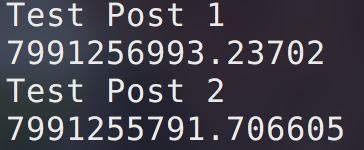
\includegraphics[scale=1]{Figures/test_time}
    \caption{Demonstration of scoring posts by time}
    \label{test_time}
\end{minipage}%
\end{figure}

As we can see from figure \ref{test_time}, Post 2 scores higher since it was created after Post 1.

In order to test the next segment of the algorithm which are common intersts, I will change the interests of Post 1 to "news" and "leisure" and keep Post 2 as is.

\begin{figure}[htbp]
\begin{minipage}[t]{\linewidth}
  \centering
    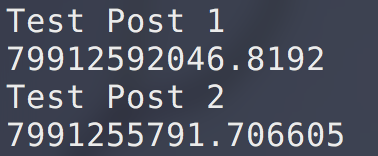
\includegraphics[scale=1]{Figures/test_common}
    \caption{Demonstration of scoring posts by common interests}
    \label{test_common}
\end{minipage}%
\end{figure}

The results are visible in figure \ref{test_common}, where even though Post 1 is older, it has one more common interest with the user, thus ranking Post 1 higher. This might not have been the case where Post 1 to be much older than Post 2.

Another element to examine is whether a post with one common and one non-common interest ranks lower than a with just one common interest.

\begin{figure}[htbp]
\begin{minipage}[t]{\linewidth}
  \centering
    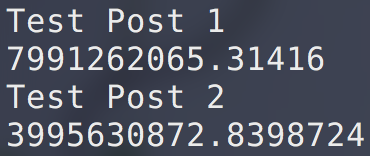
\includegraphics[scale=1]{Figures/test_non_common}
    \caption{Demonstration of scoring posts by non-common interests}
    \label{test_non_common}
\end{minipage}%
\end{figure}

Figure \ref{test_non_common} shows that Post 2 ranks much lower than Post 1 since one of the Post 1's interests are irrelevant to the user.

Lastly, in order to test the final component of the algorithm, which are penalties, I will set the same interests for both Posts but include one of the penalised words in the contents of Post 2 and leave Post 1 as is.

\begin{figure}[htbp]
\begin{minipage}[t]{\linewidth}
  \centering
    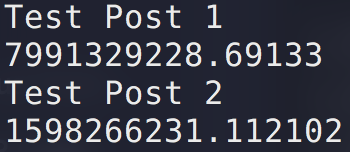
\includegraphics[scale=1]{Figures/test_penalties}
    \caption{Demonstration of scoring posts by the use of penalised words}
    \label{test_penalties}
\end{minipage}%
\end{figure}

It is clear from figue \ref{test_penalties} that the penalty deductions has indeed taken place and Post 2 is now scored lower than Post 1.
